% Options for packages loaded elsewhere
\PassOptionsToPackage{unicode}{hyperref}
\PassOptionsToPackage{hyphens}{url}
\PassOptionsToPackage{dvipsnames,svgnames,x11names}{xcolor}
%
\documentclass[
  11pt,
]{article}

\usepackage{amsmath,amssymb}
\usepackage{iftex}
\ifPDFTeX
  \usepackage[T1]{fontenc}
  \usepackage[utf8]{inputenc}
  \usepackage{textcomp} % provide euro and other symbols
\else % if luatex or xetex
  \usepackage{unicode-math}
  \defaultfontfeatures{Scale=MatchLowercase}
  \defaultfontfeatures[\rmfamily]{Ligatures=TeX,Scale=1}
\fi
\usepackage{lmodern}
\ifPDFTeX\else  
    % xetex/luatex font selection
\fi
% Use upquote if available, for straight quotes in verbatim environments
\IfFileExists{upquote.sty}{\usepackage{upquote}}{}
\IfFileExists{microtype.sty}{% use microtype if available
  \usepackage[]{microtype}
  \UseMicrotypeSet[protrusion]{basicmath} % disable protrusion for tt fonts
}{}
\makeatletter
\@ifundefined{KOMAClassName}{% if non-KOMA class
  \IfFileExists{parskip.sty}{%
    \usepackage{parskip}
  }{% else
    \setlength{\parindent}{0pt}
    \setlength{\parskip}{6pt plus 2pt minus 1pt}}
}{% if KOMA class
  \KOMAoptions{parskip=half}}
\makeatother
\usepackage{xcolor}
\usepackage[lmargin=1in,rmargin=1in,tmargin=1in,bmargin=1in]{geometry}
\setlength{\emergencystretch}{3em} % prevent overfull lines
\setcounter{secnumdepth}{3}
% Make \paragraph and \subparagraph free-standing
\makeatletter
\ifx\paragraph\undefined\else
  \let\oldparagraph\paragraph
  \renewcommand{\paragraph}{
    \@ifstar
      \xxxParagraphStar
      \xxxParagraphNoStar
  }
  \newcommand{\xxxParagraphStar}[1]{\oldparagraph*{#1}\mbox{}}
  \newcommand{\xxxParagraphNoStar}[1]{\oldparagraph{#1}\mbox{}}
\fi
\ifx\subparagraph\undefined\else
  \let\oldsubparagraph\subparagraph
  \renewcommand{\subparagraph}{
    \@ifstar
      \xxxSubParagraphStar
      \xxxSubParagraphNoStar
  }
  \newcommand{\xxxSubParagraphStar}[1]{\oldsubparagraph*{#1}\mbox{}}
  \newcommand{\xxxSubParagraphNoStar}[1]{\oldsubparagraph{#1}\mbox{}}
\fi
\makeatother


\providecommand{\tightlist}{%
  \setlength{\itemsep}{0pt}\setlength{\parskip}{0pt}}\usepackage{longtable,booktabs,array}
\usepackage{calc} % for calculating minipage widths
% Correct order of tables after \paragraph or \subparagraph
\usepackage{etoolbox}
\makeatletter
\patchcmd\longtable{\par}{\if@noskipsec\mbox{}\fi\par}{}{}
\makeatother
% Allow footnotes in longtable head/foot
\IfFileExists{footnotehyper.sty}{\usepackage{footnotehyper}}{\usepackage{footnote}}
\makesavenoteenv{longtable}
\usepackage{graphicx}
\makeatletter
\def\maxwidth{\ifdim\Gin@nat@width>\linewidth\linewidth\else\Gin@nat@width\fi}
\def\maxheight{\ifdim\Gin@nat@height>\textheight\textheight\else\Gin@nat@height\fi}
\makeatother
% Scale images if necessary, so that they will not overflow the page
% margins by default, and it is still possible to overwrite the defaults
% using explicit options in \includegraphics[width, height, ...]{}
\setkeys{Gin}{width=\maxwidth,height=\maxheight,keepaspectratio}
% Set default figure placement to htbp
\makeatletter
\def\fps@figure{htbp}
\makeatother
% definitions for citeproc citations
\NewDocumentCommand\citeproctext{}{}
\NewDocumentCommand\citeproc{mm}{%
  \begingroup\def\citeproctext{#2}\cite{#1}\endgroup}
\makeatletter
 % allow citations to break across lines
 \let\@cite@ofmt\@firstofone
 % avoid brackets around text for \cite:
 \def\@biblabel#1{}
 \def\@cite#1#2{{#1\if@tempswa , #2\fi}}
\makeatother
\newlength{\cslhangindent}
\setlength{\cslhangindent}{1.5em}
\newlength{\csllabelwidth}
\setlength{\csllabelwidth}{3em}
\newenvironment{CSLReferences}[2] % #1 hanging-indent, #2 entry-spacing
 {\begin{list}{}{%
  \setlength{\itemindent}{0pt}
  \setlength{\leftmargin}{0pt}
  \setlength{\parsep}{0pt}
  % turn on hanging indent if param 1 is 1
  \ifodd #1
   \setlength{\leftmargin}{\cslhangindent}
   \setlength{\itemindent}{-1\cslhangindent}
  \fi
  % set entry spacing
  \setlength{\itemsep}{#2\baselineskip}}}
 {\end{list}}
\usepackage{calc}
\newcommand{\CSLBlock}[1]{\hfill\break\parbox[t]{\linewidth}{\strut\ignorespaces#1\strut}}
\newcommand{\CSLLeftMargin}[1]{\parbox[t]{\csllabelwidth}{\strut#1\strut}}
\newcommand{\CSLRightInline}[1]{\parbox[t]{\linewidth - \csllabelwidth}{\strut#1\strut}}
\newcommand{\CSLIndent}[1]{\hspace{\cslhangindent}#1}

\makeatletter
\@ifpackageloaded{float}{}{\usepackage{float}}
\floatstyle{plain}
\@ifundefined{c@chapter}{\newfloat{atbl}{h}{loatbl}}{\newfloat{atbl}{h}{loatbl}[chapter]}
\floatname{atbl}{Table A}
\floatstyle{plaintop}
\restylefloat{atbl}
\newcommand*\quartoatblref[1]{Table \hyperref[#1]{A\ref{#1}}}
\@ifpackageloaded{caption}{}{\usepackage{caption}}
\DeclareCaptionLabelFormat{quartoatblreflabelformat}{#1#2}
\captionsetup[atbl]{labelformat=quartoatblreflabelformat}
\newcommand*\listofatbls{\listof{atbl}{List of Appendix Tabless}}
\makeatother
\makeatletter
\@ifpackageloaded{caption}{}{\usepackage{caption}}
\AtBeginDocument{%
\ifdefined\contentsname
  \renewcommand*\contentsname{Table of contents}
\else
  \newcommand\contentsname{Table of contents}
\fi
\ifdefined\listfigurename
  \renewcommand*\listfigurename{List of Figures}
\else
  \newcommand\listfigurename{List of Figures}
\fi
\ifdefined\listtablename
  \renewcommand*\listtablename{List of Tables}
\else
  \newcommand\listtablename{List of Tables}
\fi
\ifdefined\figurename
  \renewcommand*\figurename{Figure}
\else
  \newcommand\figurename{Figure}
\fi
\ifdefined\tablename
  \renewcommand*\tablename{Table}
\else
  \newcommand\tablename{Table}
\fi
}
\@ifpackageloaded{float}{}{\usepackage{float}}
\floatstyle{ruled}
\@ifundefined{c@chapter}{\newfloat{codelisting}{h}{lop}}{\newfloat{codelisting}{h}{lop}[chapter]}
\floatname{codelisting}{Listing}
\newcommand*\listoflistings{\listof{codelisting}{List of Listings}}
\makeatother
\makeatletter
\makeatother
\makeatletter
\@ifpackageloaded{caption}{}{\usepackage{caption}}
\@ifpackageloaded{subcaption}{}{\usepackage{subcaption}}
\makeatother
\ifLuaTeX
  \usepackage{selnolig}  % disable illegal ligatures
\fi
\usepackage{bookmark}

\IfFileExists{xurl.sty}{\usepackage{xurl}}{} % add URL line breaks if available
\urlstyle{same} % disable monospaced font for URLs
\hypersetup{
  pdftitle={The Hidden Poor: Solving Time Poverty through Redistribution of Household Production},
  pdfauthor={Fernando Rios-Avila; Aashima Sinha},
  pdfkeywords={Time Poverty, Income Poverty, Redistribution , household
production, care work, gender equality, LIMTIP},
  colorlinks=true,
  linkcolor={blue},
  filecolor={Maroon},
  citecolor={Blue},
  urlcolor={Blue},
  pdfcreator={LaTeX via pandoc}}


\usepackage{datetime}
\usepackage{booktabs}
\usepackage{chngcntr}
\usepackage{apptools}
\usepackage{lipsum}
\usepackage{booktabs}
\usepackage{multirow}
\AtAppendix{\counterwithin{table}{section}}
\AtAppendix{\counterwithin{figure}{section}}

\title{The Hidden Poor: Solving Time Poverty through Redistribution of
Household Production}
\author{
Fernando Rios-Avila\\
Levy Economics Institute\\
\\
\and 
Aashima Sinha\\
Levy Economics Institute\\
\\
}
\date{2024-06-17}
\begin{document}


\def\spacingset#1{\renewcommand{\baselinestretch}%
{#1}\small\normalsize} \spacingset{1}

%Ipsum lorem

\maketitle
\begin{abstract}
In this policy brief we start by presenting the Levy Institute measure
of Time and Income Poverty (LIMTIP) estimates for the United States from
2005 to 2023 calculated based on the statistically matched American Time
Use survey (ATUS) and Annual Social and Economic Supplements (ASEC)
data. Next, we implement redistribution simulations to explore the
potential of redistributing household production time shares, among
working-age household members, to lift individuals and hosueholds out of
time poverty. Our simulations include three scenarios based on equality,
equity and opportunity costs principles. We focus on time poor
housheolds with atleast two working-age individuals and segregate
individuals into households where everyone is time poor (HH type I);
atleast one time poor and one time-non poor individual but no scope to
bring household out of poverty (HH type II); and where time surplus of
members exceed time deficits (HH type III). We compare redistribution
scenarios based on transition rates of individuals entering and exiting
poverty across different types of time poor households. Further, we
present the relative transition rates across subgroups of gender, age,
education, employment status and presence of children. Overall, we find
across all redistribution scenarios that significant share of
individuals and households can exit time poverty, most pronounced in
equity-based redistribution and in HH type III. Moreover, time poverty
and number of hidden poor declines in all three scenarios and in all
household types except HH type II. Our analysis points towards tailoring
redistribution policies by household type and by composition of
time-poor aand time non-poor individuals. This in turn could help
support broader poverty alleviation efforts.
\end{abstract}
 
\vspace{.2in}

\textbf{\textit{Keyword: }}Time Poverty, Income Poverty, Redistribution
, household production, care work, gender equality, LIMTIP


\thispagestyle{empty}
\clearpage\pagenumbering{arabic}
\newpage
\spacingset{1.2} % DON'T change the spacing!
\section{Introduction}\label{introduction}

Redistribution of household production, which includes unpaid caregiving
and domestic chores, has been identified as an important tool to achieve
gender equality. The incorporation of the 3R (recognizition, reduction
and redistribution) strategy as a target in the United Nations
sustainable development goals, is a testament to the decades of activism
and advocacy emphasizing that gender inequality on this front cannot be
justified in the name of ``private family matter'' rather is a matter of
public policy. Redistribution can take place from households to the
public and/or private spheres, as well as among household members. While
all household members may share household work, evidence shows that it
is disproportionately undertaken by girls and women globally (Addati et
al., 2018).

Redistribution of household production responsibilities from women to
men is important intrinsically for human rights and fairness concerns,
it is also instrumental in achieving gender equality in labor market
outcomes (Bruyn-Hundt, 1996; Elso, 2017; Esquivel, 2016). Studies have
demonstrated that gender gaps in the workforce and the unequal sharing
of household responsibilities can severely impede economic growth and
development (Berik et al., 2009; Duflo, 2012; Elson, 2009). Yet, public
policies and collective actions have been less than adequate, especially
in poorer countries with constrained fiscal capacity, widespread absence
of formal wage labor and weak welfare states. Moreover, in patrirachal
contexts, cultural barriers restrict redistribution of household
production, particularly unpaid care work from women to men and to the
public and private spheres. While in some developed countries such as
Norway and Sweden public policies have been able to promote
gender-equitable sharing of household production, such as paid paternity
leaves in addition to paid maternity leaves, they have attained limited
attention and success in other countries.

The U.S. is not the exception. Issues related to lack of public
provisioning of care infrastructure and services, widespread existence
of childcare deserts, lack of paid parental leave laws among others have
gained momentum. In 2021, the value of unpaid household work in the U.S.
amounted to \$600 billion, constituting approximately 2.6\% of the GDP
(Reinhard et al., 2023). Moreover, like most other countries, we observe
gender disparity in sharing of household work such that women
disproportionately shoulder the burden. According to the 2018 American
Time Use Survey, among adults aged 15 and older, women on average spent
5.7 hours per day on unpaid household and care work, compared with 3.6
hours for men. In other words, women spent 37 percent more time on
unpaid household and care work than men (Hess et al., 2020).
Additionally, the U.S. falls behind many OECD countries in effective
childcare policies, spending only 0.4\% of GDP on early childhood
education and care (ECEC), compared to the OECD average of 0.8\% (OECD,
2020). Notably, the U.S. lacks federal laws granting paid parental
leave, setting it apart from other OECD nations. Around 51\% of the U.S.
population resides in childcare deserts, defined as census tracts with
more than 50 children under the age of 5 and either no childcare
providers or significantly limited options, resulting in a severe
shortage of licensed child care slots (Malik et al., 2018).

The lack of public provisioning of care infrastructure and services, and
the disproportionate burden of household production on women, has
implications for time poverty, both at the individual and the
household/family level. Individual time poverty refers to the lack of
time available individuals have to engage in activities that are
essential for taking care of the household, its members, self-care, and
paid work. At the household level, even if a single individual struggles
to meet his responsibilities, the whole family is considered to be
living under time poverty. In this framework, as pointed out in
(\textbf{policybrief\_USLIMTIP?}), it is not uncommon to see households
with a mixture time time availability among its members. In fact, just
over 20\% of the working age population are not time poor, but live in a
household where at least one person lives under time poverty. In spite
of the growing recognition of the importance of time constrain and the
responsibility of household production, the issue of time poverty has
received limited attention in the U.S. partially due to data
availability constraints.

Over the last decades, the Levy Economic Institute has been at the
forefront of recognizing the importance of time for understanding income
and poverty dynamics (Zacharias, 2011). As part of this work, they
developed a new measure of poverty that incorporates the dimension of
time into traditional poverty measures: The Levy Institute Measure of
Time and Income Poverty (LIMTIP for short). This measure uses synthetic
data in order to incorporate the value of time, or more specifically the
amount of resources required to outsource the responsibilities that
cannot be covered by the household members, into traditional measures of
poverty thresholds. By incorporating this dimension, the LIMTIP not only
provides a more comprehensive understanding of poverty but also allows
for the identification of the hidden poor, i.e., individuals where their
families do not have enough monetary resources to accommodate for the
time deficits they face (Antonopoulos et al., 2017; Masterson, 2012;
Zacharias et al., 2012, 2014, 2018, 2021).

While most of the earlier work on LIMTIP has focused on the analysis of
Time Poverty in developing countries (Masterson, 2012; Masterson et al.,
2022; Zacharias et al., 2018), recent work has extended the measure to
the U.S. (Zacharias et al., 2024;
\textbf{policybrief\_USLIMTIP?}).\footnote{This is in addition to the
  work done for Levy Institute Measure of Economic Well-Being (LIMEW).}.
Similar to earlier work, one of the findings of
(\textbf{policybrief\_USLIMTIP?}) is that a large share of the
population experience some level of time poverty, which translates into
a significant share of households who are \textbf{\emph{hidden poor}},
thus not captured by the official income poverty measure. However, this
work also suggests that a significant share of time poor individuals and
households could potentially exit time poverty if household production
responsibilities were to be redistributed among its members (similar to
Zacharias et al. (2021)).

Following (\textbf{policybrief\_USLIMTIP?}), this policy brief we
explore this possibility further. Using the new estimates for LIMTIP for
the U.S., we provide insights into how redistributing household
production can reduce incidence of poverty not only of individuals, but
also of the households they live in. To do this, we consider three
redistribution scenarios based on equality, equity, and opportunity
costs principles and assess the change they could have in time poverty
on working-age (18-64 years) household members.

In the next section we start with briefly describing the LIMTIP measure
and our estimates for the US. We then move on to identifying the
different types of households experiencing time poverty, the
redistribution scenarios, followed by results and policy implications.

\section{LIMTIP: A New Measure of Time Poverty for the United
States}\label{limtip-a-new-measure-of-time-poverty-for-the-united-states}

Poverty is a multidimensional concept that goes beyond the simple notion
of lack of income. In addition to income, poverty can be understood as a
lack of access to resources, including time. The LIMTIP is a metric
that, in addition to income poverty, incorporates aspects of time
poverty that better captures the control household have on their
resources. In this framework, time poverty refers to a scenario wherein
people may not have any time left after engaging in activities that are
essential for taking care of the household, its members, self-care, and
paid work. At the household level, we consider an even more restrictive
definition. Under the assumption that individuals with time surpluses
are unable or unwilling to help those with time deficits, we consider a
household to be time poor if at least one member is time poor.

As described in (\textbf{policybrief\_USLIMTIP?}) and
(\textbf{wp\_qmatch?}), the LIMTIP is built using a synthetic dataset
that combines information from the American Time Use Survey (ATUS) and
the Annual Social and Economic Supplements (ASEC) of the Current
Population Survey (CPS). For the identification of time poverty, using
weekly hours as unit of analysis (168hrs per week), we identify the
amount of time individuals would have left (\(X_{ij}\)) after engaging
in required activities for taking care of their share of
responsabilities (\(\alpha_{ij}\)) taking care of the household and its
members (\(R_j\)), personal maintenance (\(M\)), and paid work
(Commuting \(T_{ij}\) and time spent at work \(T_{ij}\)). This is
expressed in the following equation (see Equation~\ref{eq-bal}):

\begin{equation}\phantomsection\label{eq-bal}{X_{ij} = 168 - M - \alpha_{ij}R_j-D_{ij}(L_{ij}+T_{ij})
}\end{equation}

The minimum time required for each of the components in
Equation~\ref{eq-bal} are estimated using a mixture of assumptions, the
synthetic dataset and the ATUS dataset (see (\textbf{wp\_qmatch?}) for
details).

At the household level, however, we assume that individuals with time
surpluses are unable or unwilling to share and redistribute some of the
responsabilities of those with time deficits. In this framework, a
household is considered to be time poor as long as there is one person
with time deficit living in the household.\footnote{To identify time
  poverty status, we only consider the time deficits of household
  members age 18 or older.} This is expressed in the following equation
(see Equation~\ref{eq-hbal}):

\begin{equation}\phantomsection\label{eq-hbal}{X_{j} = \sum_{i=1}^{I_j} \min(X_{ij},0)
}\end{equation}

Once household time deficits are identified, we can adjust the official
income poverty thresholds to account for time deficits, after monetizing
its value. For the U.S. case, we use a three-year average hourly wages
for the industry private households obtained from Merged Outgoing
Rotation Groups (MORG) to value the household time deficit. This value
represents the amount of income may be required to outsource some of the
time responsabilities, and eliminate time poverty. The adjusted poverty
line, and the LIMTIP, is then calculated as:

\begin{equation}\phantomsection\label{eq-limtip}{Z_{j}^{adj} = Z_{j} + 52*wage* |X_{j}|
}\end{equation}

where \(wage\) is the price we use to give a monetary value to the time
deficits the household \({j}\) faces, and \(Z_{j}^{adj}\) is the
adjusted poverty line. Intuitively, households that are not time poor
will not chance status compared to the official poverty estimates.
However, households that are time poor could have their poverty status
change if, after considering the adjusted poverty line, they fall below
it. This group of households are considered to be the hidden poor.

\begin{table}

\caption{\label{tbl-limtip}4-Way Classification Based on Time and Income
Poverty: LIMTIP}

\begin{minipage}{0.50\linewidth}

\subcaption{\label{tbl-limtip1}Individuals}

\centering{

 
  \centering
  \begin{tabular}{lcccc}
    \toprule
    & \multicolumn{2}{c}{Income Poverty} & \multirow{2}{*}{Total} \\
                   & Poor   & Non-Poor &        \\
    \midrule
    Time Poverty   &        &          &        \\
    \quad Poor     & 3.5\% & 21.7\%   & 25.2\%  \\
    \quad Non-Poor & 11.9\% & 62.9\%   & 74.8\% \\
    \cmidrule{1-4}
    Total          & 15.4\% & 84.6\%   & 100\%  \\
    \bottomrule
  \end{tabular}

}

\end{minipage}%
%
\begin{minipage}{0.50\linewidth}

\subcaption{\label{tbl-limtip2}Households}

\centering{

 
  \centering
  \begin{tabular}{lcccc}
    \toprule
    & \multicolumn{2}{c}{Income Poverty} & \multirow{2}{*}{Total} \\
                   & Poor   & Non-Poor &        \\
    \midrule
    Time Poverty   &        &          &        \\
    \quad Poor     & 6.0\% & 39.4\%   & 45.4\%  \\
    \quad Non-Poor & 9.8\% & 44.8\%   & 55.6\% \\
    \cmidrule{1-4}
    Total          & 15.8\% & 84.2\%   & 100\%  \\
    \bottomrule
  \end{tabular}

}

\end{minipage}%

\end{table}%

Using this information, it is possible to classify individuals (and
households) into four categories based on their time and income poverty
status. In Table~\ref{tbl-limtip}, we present the averaged shares of
individuals across years 2005 to 2023. By construction, individuals
living in non-time poor households will face the same poverty status as
the official poverty estimates, because the poverty line is not
adjusted. Thus, they are of little interest to us. Instead, our focus is
on individuals living in time poor households, because they are the ones
where the hidden poor are to be found. Based on the information in
Table~\ref{tbl-limtip}, whereas 25.2\% of individuals are time poor,
45.4\% of individuals live in time poor households. This implies that
there is a lot of scope for redistribution of household production
responsibilities among working-age members to lift individuals and
households out of time poverty.

Across the years of available data, individual level time poverty has
shown a small increasing trend from 2008 to 2023 from about 21.4\% to
25.0\% (see Figure~\ref{fig-trend}). Perhaps the most notable change
across years has been the sudden decrease in time poverty in 2020, which
is likely due to the pandemic and the lockdowns that followed. Over the
same period the official poverty estimates shows a slight rising trend
between 2005 to 2014 and then starts to decline, with the exception of
2023. When we adjust for time deficits, the LIMTIP estimates shows a
higher level of poverty across all years, around 3-5 percentage points
higher, wich represent the hidden poor.

Overall, while some trends can be observed in terms of time and income
poverty, the changes have been relatively small. This suggests that the
problems related to time poverty and the hidden poor are persistent, but
show little hettrogeinity across years. Because of this, the rest of
this policy brief will focus on average results across all years.

\begin{figure}[H]

\centering{

\includegraphics{resources/trend.pdf}

}

\caption{\label{fig-trend}Trends of Time, Income and Limtip Poverty in
the U.S.}

\end{figure}%

\section{Identifying the Problem}\label{sec-problem}

As suggested earlier, one of the strategies that could help reduce the
problem of time poverty, and thereby the incidence of hidden poor, is
the redistribution of household production responsibilities across all
working age members in the household. At best, household members with
time surpluses could take on more household responsabilities, reducing
the burden of those with time deficits, and potentially lifting out
household out of poverty. At worst, the redistribution could make the
time deficits more equal among the household members, even if the
household remains time poor.

Before we start analyzing the potential that redistribution could have
in reducing time poverty, we must first identify the households where
redistribution is possible. Specifically, we exclude from the analysis
households that are not time poor, because the goal of the of the
current analysis is to evaluate the potential of redistribution in
lifting individuals and households out of time poverty. While non-time
poor households could potentially benefit from redistribution, reducing
the gaps of time surpluses among household members, resulting in more
gender-equitable sharing of household work, this second order effect is
beyond the current scope of this policy brief.

From the sample of individuals living in a time poor household we
classify them into five different groups:

\begin{itemize}
\tightlist
\item
  \textbf{Single}: These are time poor individuals that live in a
  household where they are the only working-age person. In this case,
  redistribution is not possible, and thus are excluded from the
  analysis.
\item
  \textbf{Time Poor in H. Type I}: These are time poor individuals who
  live in households where all working-age members are time poor. While
  redistribution is possible, and may help in reducing the time deficits
  of some individuals, and even allow some to transition out of time
  poverty, the household will remain time poor regardless of the
  redistributional scenario.
\item
  \textbf{Time Poor in H. Type II}: These are time poor individuals who
  live in households where there are non-time poor members. However, the
  combined time surpluses is insufficient to lift the household out of
  time poverty.
\item
  \textbf{Time Poor in H. Type III}: These are time poor individuals who
  live in households where there is enough time surplus to lift the
  household out of time poverty. Redistribution in these households can
  lift all working members of the household out of time poverty.
\item
  \textbf{Non Time poor in a Time Poor household}: This last group
  consists of individuals with time surpluses living in a time poor
  household. The goal of the redistribution scenarios is to allocate
  household responsabilities in such a way that these invididuals can
  help lift other household members out of time poverty. However, it is
  also possible that some of these individuals may end up experiencing
  time poverty in the redistribution scenarios.
\end{itemize}

Figure~\ref{fig-composition} provides a visual representation of the
classification of working age individuals (18-64yrs of age) living in
time poor households across the years. As it can be observed, about 40\%
of individuals were living in a time poor household. While this share
shows a sharp increase between 2005 and 2007, it has remained stable
from 2008 onwards, with a small increase across years that mimics the
raise of individual time poverty observed in Figure~\ref{fig-trend}.
There is an additional 4-5\% of individuals who are time poor but
redistribution is not possible. From the rest, about 15\% of individuals
constitute our main group of analysis, i.e., those living in households
where redistribution may be sufficient to lift the household out of time
poverty. The remaining 20\% are individuals who are not time poor but
live in a time poor household.

\begin{figure}[H]

\centering{

\includegraphics{resources/tpov_type.pdf}

\footnotesize

\begin{flushleft}Note: T.P.H.: Time Poor Household, H.Type I : All working age members are time poor, H.Type II: There are Non-time poor individuals Living in the HH, but time surplus is insufficient to Lift HH out of Time poverty, H.Type III: There is enough time surplus to lift HH out of time poverty.\end{flushleft}

}

\caption{\label{fig-composition}Time Poverty classification, across
time}

\end{figure}%

In the next section, we discuss three redistribution scenarios wherein
household responsabilities can be redistributed among working-age
members, under different criteria. Nevertheless, we should keep in mind
that we will only be analyzing the impact of redistribution on time poor
households with at least 2 working-age members.

\section{Redistribution Scenarios}\label{redistribution-scenarios}

The idea of redistribution of household production responsibilities
follows the principle that everyone in a household should be able to
carry out their \textbf{fair} share of household work. The question,
however, is what constitutes a fair share?. In this section we present
three different principles that could guide the redistribution of
household production responsibilities among working-age members.

First, we use the simple egalitarianism principle that involves an equal
division of total household production time among all working age
members. Second, we redistribute conditional on the time available to
people. Finally, in the third scenario, redistribution is guided based
on the principle of opportunity cost of time, where those with higher
wages (higher opportunity cost of time) are assigned less household
production time.

For all scenarios, we only consider the redistribution of required
household production activities \(R_j\) net of the portion met by other
household members. Thus, the goal of the different scenarios is to
simulate different \(\alpha_{ij}\) values, which represent the share of
required household production time that each household member takes on.
We also impose the assumption that all household members are equally
efficient at taking care of the household responsabilities. We outline
the methods used for implementing the scenarios below.

\subsection{Scenario 1: Equal Shares}\label{scenario-1-equal-shares}

The first scenario considers the impact of redistributing household
production such that all working-age members of the household are
assigned an equal share of the required household production time. The
new share is defined as:

\begin{equation}\phantomsection\label{eq-r1}{\alpha_{ij}^E= \frac{1}{I_j}*(1-\alpha_{j}^{nw})
}\end{equation}

where \(\alpha_{ij}^E\) represents the redistributed share of individual
\(i\); \(I^j\) is the number of working-age persons in household \(j\)
and \(\alpha_{j}^{nw}\) represents the total share of all non-working
age household members. While this principle aligns with the idea of
equality, it overlooks time equity, by redistribution tasks without
taking into consideration the time available of individuals.

\subsection{Scenario 2: Time Available}\label{scenario-2-time-available}

The time available scenario is based on the principles of equity. In
contrast with Scenario 1, this one suggests that household
responsabilities could be redistributed relative to the available time
individuals may have after setting aside the time for personal
maintenance requirements and income generation
(\(Z_{ij}=168-M-D_{ij}(L_{ij}+T_{ij})\)).

To implement this first we calculate the time available (\(Z_{ij}\)) for
each individual, and recalculate the shares \(\alpha_{ij}^A\), using the
ratio of time available to the total time available among working-age
members. For individuals that do not have any time available
(\(Z_{ij}<0\)), we set their \(Z_{ij}\) to zero. This ensures that
people who already suffer from time povery are not assigned further
tasks within the household. The new share is defined as:

\begin{equation}\phantomsection\label{eq-r2}{
\begin{aligned}
Z_{ij} &=\max{\Big(168-M-D_{ij}(L_{ij}+T_{ij}),0\Big)} \\
\alpha_{ij}^A &= \frac{Z_{ij}}{\sum Z_{ij}} (1-\alpha_{j}^{nw})
\end{aligned}
}\end{equation}

Because there are individuals (young adults) who may still be in school,
the standard definition of \(Z_{ij}\) may not capture their true time
availability. To address this we add a correction to time availability
to all individuals who declared to attend school, using the average
number of hours people spend in education activities per week. This
correction does not affect the time balance used for the identification
of the time poor, only the estimation of the adjusted shares
\(\alpha_{ij}^A\).

\subsection{Scenario 3: Opportunity
Cost}\label{scenario-3-opportunity-cost}

The third possibility is based on the idea of opportunity costs along
marginalist lines. The sharing rule depends on the earning potentials of
individuals, such that individuals with higher potential wages are
assigned a lower share of household production time. In principle, this
would encourage the most productive members of the household to spend
more time in paid work, while those with lower earning potentials would
take on more household production responsibilities.

For example, if there are only three working-age adults in a household,
and where the secpmd member earns twice as much as the first, and the
third earns three times as much as the first, the shares of household
production would be 1/2, 1/3, and 1/6 respectively. To implement this
scenario, we first calculate the inverse of the wage of each individual
\(rw_{ij}\), rescale it to sum to 1, and then calculate the share of
household production time as follows:

\begin{equation}\phantomsection\label{eq-r3}{\begin{aligned}
rw_{ij} &= \frac{1}{w_{ij}} \\
\alpha_{ij}^O &= \frac{rw_{ij}}{\sum rw_{ij}} (1-\alpha_{j}^{nw})
\end{aligned}
}\end{equation}

where \(w_{ij}\) is the wage of individual \(i\).

Because we do not have wage data for non-working household members, we
use the potential/predicted wages for all working-age household members.
To do this, we use a two-step procedure. First, we predict occupation
and industry probabilities for all non-working individuals using a
multinomial logit model. Second, we estimate a maximum likelihood
Heckman selection model (Heckman, 1979) using the observed and predicted
probabilities of belonging to specific occupations and industries, in
addition to individual, household and spouse demographic
characteristics. With this information, we predict wages based on the
model that corrects for sample selection.

\section{Results}\label{results}

As described in the previous section, we consider three scenarios to
analyze the impact that redistribution could have on time poverty,
focusing on individuals living in time poor households with at least two
working-age members. In this section, we present the results of the
redistribution scenarios and discuss the implications for time poverty
and the incidence of hidden poor. Specifically, we analyze how effective
are the redistribution scenarios in helping time poor individuals exit
time poverty, as well as to what extend non-time poor individuals are
affected by the redistribution scenarios, falling into time poverty. We
refer to both of these as transition rates (into and out of time
poverty). Since most of the results across time are similar, we focus on
providing results that average the impacts of redistribution across all
years.

\subsection{Redistribution Scenarios and Time Poverty: General
Results}\label{redistribution-scenarios-and-time-poverty-general-results}

Figure~\ref{fig-dist} provides the distribution of individuals, and
their households by type. Figure~\ref{fig-dista} shows that 54.6\%
individuals live in time poor households are not time poor themselves.
These are the individuals that could help lift other household members
out of time poverty, by taking on more household responsibilities.

From the rest, 4.6\% live in households where everyone is time poor (HH
Type I), 7.1\% live in households with at least one not-time-poor
individual, but with insufficient time surplus to lift the household out
of time poverty (HH type II), and 33.7\% live in households where there
is enough time surplus to lift every household member out of poverty (HH
type III). It is important to note, that only in househodl type III,
redistributon could be helpful in lifting the entire housheold out of
poverty.

In terms of household structure, Figure~\ref{fig-distb} shows 81.2\% of
the households could exit from time poverty, but the remaining 18.8\%
cannot do so, even if all working-age members were to take on more
household responsibilities. This is because total household surplus is
insufficient to overcome total hosuehold deficit. Nevertheless, it may
be possible to reduce the time deficits of some individuals in housheold
type II by reducing the time surplus of other members.

\begin{figure}[H]

\centering{

\begin{figure}[H]

\begin{minipage}{0.50\linewidth}

\centering{

\includegraphics{resources/ind_dist.pdf}

}

\subcaption{\label{fig-dista}Individuals}

\end{minipage}%
%
\begin{minipage}{0.50\linewidth}

\centering{

\includegraphics{resources/hh_dist.pdf}

}

\subcaption{\label{fig-distb}Households}

\end{minipage}%

\end{figure}%

\footnotesize

\begin{flushleft}Note: H.Type I : All working age members are time poor, H.Type II: There are Non-time poor individuals Living in the HH, but time surplus is insufficient to Lift HH out of Time poverty, H.Type III: There is enough time surplus to lift HH out of time poverty.\end{flushleft}

}

\caption{\label{fig-dist}Distribution of individuals by type}

\end{figure}%

To understand the impact of redistribution simulation on these differnt
types of household categories, across the three diferent scenarios, we
will focus on transition rates (i.e the share of individuals who can
exit or enter time poverty as a result of redistribution simulation). We
will focus on individual experiences first. For individuals who are
currently not time poor, the statistic of interest would be the share of
individuals that fall into time poverty, whereas for time poor
individuals, we will consider their poverty exit rate.

\begin{figure}[H]

\centering{

\includegraphics{resources/trans1.pdf}

}

\caption{\label{fig-transition1}Transition rates by Redistribution
Scenario}

\end{figure}%

As observed in Figure~\ref{fig-transition1}, because all the
redistribution scenarios are designed to redistribute household
production responsibilities, without avoiding putting some individuals
in time poverty, we observe that 12.3-12.9\% of non time poor
individuals will fall into time poverty across scenarios. While these
probabilities is considerably similar across scenarios, its may not be
the case that the same individuals are affected (see
Figure~\ref{fig-tran_by_group1} and Figure~\ref{fig-tran_by_group2}).

For the rest of the household categories, we observe that there are
substantially more heterogeneity on the impact of time povery across the
different scenarios. For individuals in households where all members are
time poor, the equal share and opportunity cost scenarios suggest that
up to 17\%-18\% of individuals could exist time poverty, with the lowest
exit rate (2.5\%) under Scenario 2 (time availability scenario). The
transition rates slighlty increase in the second category of housholds
with similar trend across scenarios.

Further, we observe that the transition rates are highest among HH type
III , and within these type of households, in Scenario 2 compared to
scenarios 1 and 2. This implies that in case where housheold's aggregate
time surplus exceeds household's aggregate time deficits, equity-based
principle of redistribution would allow for the highest rate of exiting
poverty. The same principle maintains much lower transition rates in the
other two household types where any decline in an individual's time
deficit could result in pushing other individuals further into time
poverty. Therefore, a lower share of individuals end up exiting poverty.

In sum, redistribution can be most effective in terms of helping people
exit poverty, among household type III, with the highest exit rates in
Scenario 2 followed by scenarios 1 and 3. On the other hand, opportunity
cost principle (Scenario 3) can allow more people exit poverty in
household types 1 and 2.

In terms of time deficits, as shown in Figure~\ref{fig-def1}, the
average time deficits (in hours per week) that non-time poor individuals
face is quite small, just around 0.7 hours. However, those who become
time poor (non-zero time deficit), their time deficits increase in the
range of 4.4-5.8 hours (see Figure~\ref{fig-def2}). Interestingly,for
this subgroup, the Time availability Scenario (Scenario 2) has the
lowest (negative) impact in moving non-time poor people enter time
poverty by increasing their time deficits.

While such a case may suggest an improvement on the quality of life of
some individuals, the redistribution scenarios also have implications in
terms of time deficits other household members face. As shown in
Figure~\ref{fig-def1}, average time deficit increase in roughly 1 hour
for scenarios 1 and 3. However, as shown in Figure~\ref{fig-def2}, the
time deficit for those who remain time poor increase in just over 3hrs.
In general, while the availability scenario has smallest impact on
transition rates, it also has the smallest impact in terms of time
deficits, for those who remain time poor. !! AS to check again not
clear!!

\begin{figure}[H]

\centering{

\centering{

\includegraphics{resources/def1.pdf}

}

\subcaption{\label{fig-def1}Average Time Deficits}

\centering{

\includegraphics{resources/def2.pdf}

}

\subcaption{\label{fig-def2}Average Time Deficits (Excluding Zeros)}

}

\caption{\label{fig-deficit}Time Deficits across Scenarios}

\end{figure}%

The next group of interest are those individual living in households
that cannot exit time poverty, but could reduce time deficits for some
of their members (Household Type II). Interestingly, the poverty exit
rates for these individuals are ver similar as for the previous group,
with the time availability scenario having the lowest impact at 8.1\%.
In contrast, when we pay attention to the time deficits, its the equal
share scenario that has the largest impact on time deficit.

At baseline, individuals in this group had in average a time deficit of
20hrs per week. Under Scenarios 1 and 3, the average deficit reduces to
9hrs and 10hrs respectively. However, under Scenario 2, it reduces to
only 5.6hrs a week. While the time availability scenario is not as
effective in reducing time poverty, it may appear it is the most fair,
as it redistributes both the gains and losses of time allocation more
equally across household members.

The last group of interest are those individuals living in households
where redistribution could lift all members out of time poverty. In this
case, all redistribution scenarios do an excellent job at reducing time
poverty, with exit rates of 72-89\%. In contrast with the two previous
cases, the time availability scenario has the largest impact reducing
time poverty, with an exit rate of 89\%. In terms of time deficits,
given the success the redistribution scenarios have in reducing time
poverty, the average time deficits is reduced to 0.4-2.3hrs per week.
However, for those who remain time poor, the impacts in terms of time
deficits are much smaller, with scenario 2 still representing the most
efficient, reducing the deficit to just 4hrs per week.

As it would be expected, this reduction in individual time poverty also
has an impact at the household. While non of the households Type I or II
are able exit time poverty, as shown in Figure~\ref{fig-transition2},
between 65-87\% of households Type III are able to exit time poverty,
with Scenario 2 being the best at reducing time poverty.

\begin{figure}[H]

\centering{

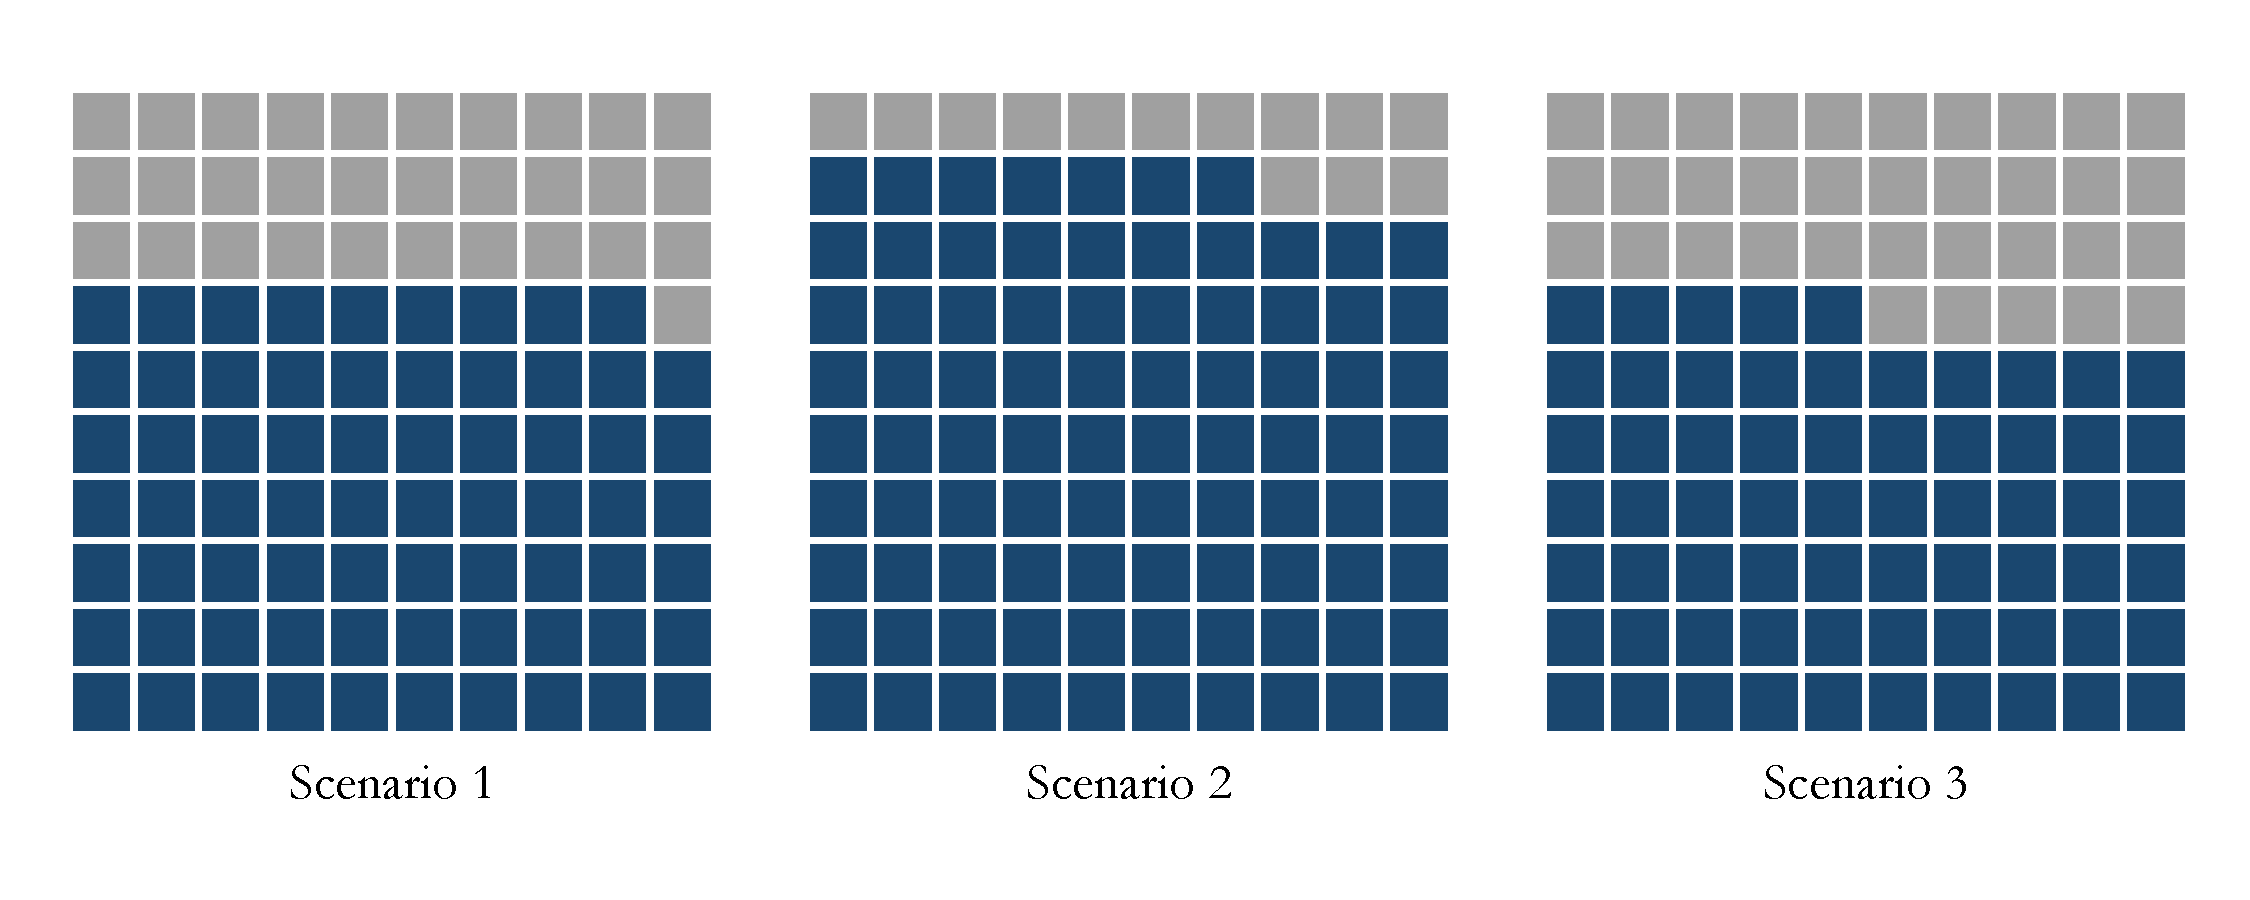
\includegraphics[width=0.7\textwidth,height=\textheight]{resources/hhtrans.pdf}

}

\caption{\label{fig-transition2}Transition probabilities for households}

\end{figure}%

\subsection{Redistribution Scenarios and Time Poverty:
Heterogeneity}\label{redistribution-scenarios-and-time-poverty-heterogeneity}

As suggested earlier, not all individuals were affected in the same way
by the redistribution scenarios. For example, groups who are
traditionally more vulnerable to time poverty, are also the most likely
to benefit from intra household redistribution of responsabilities. To
explore this further, in this section we present how the poverty
transition rates varies across different groups of individuals.
Figure~\ref{fig-tran_by_group1} and Figure~\ref{fig-tran_by_group2}
present the difference between the group specific transition rate
compares to the overall transition rate.

Under Scenarios 1 and 2, men have a higher probability of falling into
time poverty compared to women, with a lower probability of exiting time
poverty. This is particularly pronouced among individuals living in
type-III households. Interestingly, Scenario 3, which is based on
opportunity costs, shows the opposite pattern. Although we have shown
that all scenarios help reduce time poverty, the opportunity cost
scenario seem to attenuate the effect by perpetuating the gender roles
tied to earning potentials.

A second characteristics that tends to drive differences in time poverty
is related to the presence of Children. In our results, however, their
presence has mixed impact oon tn transition rates. Under all scenarios,
not time poor individuals living in households with children are more
like to fall into time poverty. However having children also increases
the chances of exiting time poverty in Household Type II, while reducing
it in Household Type III. The time availability scenario is the only
case where the results are consistent across all household types, with
children increasing the probability of falling into time poverty, but
decreasing the probability of exiting time poverty.

The last group of interst considered in Figure~\ref{fig-tran_by_group1}
is based on employment status. Since time poverty is closely related to
the time spent on paid work, we should emphasize that the share of time
poor individuals among the not employed is much smaller compared to the
employed. Because of this, the unemployed have an almost 0\% probability
of falling into time poverty, and those who are time poor, are far more
likely exit time poverty. Among the employed, while they are somewhat
more likely to fall into time poverty than average, there are almost no
singificant differences in any other scenario.

\begin{figure}[H]

\centering{

\includegraphics{resources/det1.pdf}

\footnotesize

\begin{flushleft}Note: The figure presents the difference between the group specific transition rate and the overall transition rate.\end{flushleft}

}

\caption{\label{fig-tran_by_group1}Transition probabilities
Heterogeneity: Gender, Employment Status and Children Presence}

\end{figure}%

In terms of education and age (see Figure~\ref{fig-tran_by_group2}) the
patterns are less clear. Among non time poor individuals, those with
higher levels of education seem to be the most likely to fall into time
poverty. This pattern is observed for all scenarios, with but with a
smaller impact under the opportunity cost scenario.

For time poor individuals, the patterns are less clear. When
redistribution is driven by oppotunity cost, higher levels of education
increase the probability of exiting time poverty. However, the magnitude
of the diferences is small for type III households. For Scenarios 1 and
2, we can only observe some patterns for individuals living in type III
households, where higher education reduce, rather than increase, the
probability of exiting time poverty.

Finally, in terms of age, both the youngest and oldest individuals are
less likely to fall into poverty, while also being the more likely to
exit time poverty. This patterns may be a reflection that individuals in
the age group 30-45 are most likely to be in the labor market, and thus
are less flexible in terms of time allocation, and thus are less likely
to be affected by the redistribution scenarios.

\begin{figure}[H]

\centering{

\includegraphics{resources/det2.pdf}

\footnotesize

\begin{flushleft}Note: The figure presents the difference between the group specific transition rate and the overall transition rate.\end{flushleft}

}

\caption{\label{fig-tran_by_group2}Transition probabilities
Heterogeneity: Education and Age}

\end{figure}%

\subsection{Changes in LIMTIP: The hidden
poor}\label{changes-in-limtip-the-hidden-poor}

WHile the discussion above provides a detailed picture of the potential
impact that redistribution could have on time poverty, it is equally
important to understand changes in terms of Adjusted LIMTIP estimates.

\begin{figure}[H]

\centering{

\includegraphics{resources/glimtip.pdf}

}

\caption{\label{fig-limtip}Changes in LIMTIP estimates across
redistribution scenarios}

\end{figure}%

In Figure~\ref{fig-limtip} we present the poverty rates across the
different redistribution scenarios, for the sample of households that we
identify to be time poor. The first thing to consider here is that the
incidence of official poverty and LIMTIP poverty in the sample is lower
than the one observed in the general population
(Figure~\ref{fig-trend}). This is expected, since our sample of interest
is restricted to time poor households, who are more likely to have
members working, and hence less likely to be income poor.

Even in this sample we observe a large difference between the official
poverty estimates and the LIMTIP estimates. While the official poverty
estimates are around 5\%, the LIMTIP estimates poverty to be closer to
11\%, showing that 6\% of the individuals in the sample are hidden poor.
Given the success of the redistribution scenarios in reducing time
poverty, we observe that the LIMTIP estimates are also reduced, with the
time availability scenario showing the largest reduction in poverty
rates, practically eliminating the incidence of hidden poor in the
sample.

However, a detailed look across individuals suggests that such large
improvements are not uniform across all groups. In households where all
individuals are time poor, the redistribution scenarios worsen the
poverty rates, albeit the impact is small. This happens because the
aggregated time deficit of the household increases as some individuals
who exit time poverty status. For households with some potential to
reduce aggregated time deficits (H.Type II), we observe that the share
of the hidden poor is greatly reduced from 8\% to 3 to 5\%.

\section{Policy implications}\label{policy-implications}

Intra-household redistribution of household production could serve as en
effective tool to reduce some individuals' time deficits and bring them
out of time poverty. In addition, such redistributions could have
well-being effects for the household as a whole in terms of more
equitable sharing of household production and even lifting households
out of poverty

However, redistribution policy intervention to address time poverty
would depend on household type, which would determine if only some
individuals could exit time poverty or if there is enough time surplus
to absorb time deficits, lifting the entire households out of poverty.
Redistribution policy may not be effective in a household where everyone
is time poor, infact it may end up increasing their LIMTIP poverty if
nothing else. At best, it could allow for redistributing household
production in a more equitable manner, however will not be able to bring
households out of poverty. In such a case, the extent of time deficit
experienced by individuals becomes important. Therefore, redistribution
policies need to be tailored by type of household.

In this policy brief we segregated individuals by household type and
presented how redistribution would play differently across these groups.
Further, we assessed the impact across three different redistribution
scenarios for household type. We find that all three redistribution
principles signifantly allow people to exit poverty, partiuclarly in the
type of households where the aggregate time surplus is greater than
aggregate time deficits. We observed that the equity-based
redistribution scenario serve as the most effective principle in lifting
people out of poverty and in reducing poverty rate. !!add more on
comparing the scenarios!!

Further, as the objective of estimating LIMTIP among other things is to
make the hidden poor visible, the redistribtion strategies proposed in
this brief can potentially help solve the problem of hidden poor by
reducing their time deficits and their time-adjusted poverty. The hidden
poor are invisble in the offial poverty estimates, hence do not benefit
from poverty welfare programs. Redistribution policy can help reduce the
incidence of poverty for this group. We find that in all the
redistribution scenarios the number of hidden poor declined and infact
in the equity-based scenario, to a lage extent the hidden poor were
eliminated.

While, examining redistribution among all working-age (18-64 years)
members have merit in providing an overview of the potential of
redistribution, it may end up redistributing household prodution time to
youth or school/college going students as well as to those who are older
(close to 64 years). Redistributing to these subgroups, may not be the
most ideal situtaion as it could interupt with human capacity building
by disrupting indviduals' education and health outcomes. Moreover, from
an efficieny point of of view, these subgroups may be less efficient
compared to other adults in the household. In this regard, our analysis
opens door for further examining redistribution between men and women
and focussing it on specific age-groups and even the intersection of the
two. Such targeted redistribution policies would allow moving closer to
achieving gender-equitable distribution of unpaid work

While intra-household reditribution is crucial, the role of
redistributing some of the components of housheold production,
particulary unpaid care work to the public sector cannot be overlooked.
The role of the public sector needs to expand in terms of supporting
some of the social reporoduction needs of the household, to balance
individuals' time constraints, particulalry for those in income poor
households.

A time-adjusted measure of poverty is an effort to provide evidence on
the crucial aspects of time poverty and a push towards devising public
policies to address constraints associated with time resources in
addition to income resources.

!!BTW who will enforce redistribution policy??!!

\section{Conclusion}\label{conclusion}

\section*{References}\label{sec-ref}
\addcontentsline{toc}{section}{References}

\phantomsection\label{refs}
\begin{CSLReferences}{1}{0}
\bibitem[\citeproctext]{ref-addati2018}
Addati, L., Cattaneo, U., Esquivel, V., and Valarino, I. (2018).
\emph{Care work and care jobs for the future of decent work}.
International Labour Organisation (ILO).

\bibitem[\citeproctext]{ref-Antonopoulos2017}
Antonopoulos, R., Esquivel, V., Masterson, T., and Zacharias, A. (2017).
Time and income poverty in the city of buenos aires. In R. Connelly and
E. Kongar (Eds.), \emph{Gender and time use in a global context: The
economics of employment and unpaid labor} (pp. 161--192). Palgrave
Macmillan US. \url{https://doi.org/10.1057/978-1-137-56837-3_7}

\bibitem[\citeproctext]{ref-berik2009}
Berik, G., Rodgers, Y. van der M., and Seguino, S. (2009). Feminist
{Economics} of {Inequality}, {Development}, and {Growth}. \emph{Feminist
Economics}, \emph{15}(3), 1--33.
\url{https://ezprox.bard.edu/login?url=https://search.ebscohost.com/login.aspx?direct=true&db=ecn&AN=1063369&site=eds-live&scope=site}

\bibitem[\citeproctext]{ref-hundt1996}
Bruyn-Hundt, M. (1996). Scenarios for a redistribution of unpaid work in
the netherlands. \emph{Feminist Economics}, \emph{2}(3), 129--133.
\url{https://doi.org/10.1080/13545709610001707826}

\bibitem[\citeproctext]{ref-duflo2012}
Duflo, E. (2012). Women {Empowerment} and {Economic} {Development}.
\emph{Journal of Economic Literature}, \emph{50}(4), 1051--1079.
\url{https://doi.org/10.1257/jel.50.4.1051}

\bibitem[\citeproctext]{ref-elson2017}
Elso, D. (2017). \emph{Recognize, {Reduce}, and {Redistribute} {Unpaid}
{Care} {Work}: {How} to {Close} the {Gender} {Gap}}.
\url{https://doi.org/10.1177/1095796017700135}

\bibitem[\citeproctext]{ref-elson2009}
Elson, D. (2009). Gender {Equality} and {Economic} {Growth} in the
{World} {Bank} {World} {Development} {Report} 2006. \emph{Feminist
Economics}, \emph{15}(3), 35--59.
\url{https://doi.org/10.1080/13545700902964303}

\bibitem[\citeproctext]{ref-valeria2016}
Esquivel, V. (2016). Power and the {Sustainable} {Development} {Goals}:
A feminist analysis. \emph{Gender \& Development}, \emph{24}(1), 9--23.
\url{https://doi.org/10.1080/13552074.2016.1147872}

\bibitem[\citeproctext]{ref-heckman1979}
Heckman, J. J. (1979). Sample selection bias as a specification error.
\emph{Econometrica}, \emph{47}(1), 153.
\url{https://doi.org/10.2307/1912352}

\bibitem[\citeproctext]{ref-hess2020}
Hess, Cynthia, Ahmed, T., and Hayes, J. (2020). \emph{Providing {Unpaid}
{Household} and {Care} {Work} in the {United} {States}: {Uncovering}
{Inequality}}.

\bibitem[\citeproctext]{ref-malik2018}
Malik, R., Hamm, K., Schochet, L., Novoa, C., Workman, S., and
Jessen-Howard, S. (2018). America's {Child} {Care} {Deserts} in 2018.
\emph{Center for American Progress}.
\url{https://www.americanprogress.org/article/americas-child-care-deserts-2018/}

\bibitem[\citeproctext]{ref-masterson2012}
Masterson, T. (2012). \emph{Simulations of full-time employment and
household work in the levy institute measure of time and income poverty
(LIMTIP) for argentina, chile, and mexico} (Working Paper 727; Levy
Economics Institute Working Paper). Levy Economics Institute of Bard
College.

\bibitem[\citeproctext]{ref-masterspm2022}
Masterson, T., Antonopoulos, R., Nassif-Pires, L., Rios-Avila, F., and
Zacharias, A. (2022). \emph{Assessing the impact of childcare expansion
in mexico: Time use, employment, and poverty} {[}Research Project
Report{]}. Levy Economics Institute of Bard College.
\url{https://www.levyinstitute.org/pubs/rpr_6_22.pdf}

\bibitem[\citeproctext]{ref-oecd2020}
OECD. (2020). \emph{Early learning and child well-being in the united
states} (p. 124).
https://doi.org/\url{https://doi.org/https://doi.org/10.1787/198d8c99-en}

\bibitem[\citeproctext]{ref-rein2023}
Reinhard, S. C., Caldera, S., Houser, A., and Choula, R. (2023).
\emph{Valuing the {Invaluable}: 2023 {Update}}. AARP Public Policy
Institute. \url{https://doi.org/10.26419/ppi.00082.006}

\bibitem[\citeproctext]{ref-zacharias2011}
Zacharias, A. (2011). \emph{The measurement of time and income poverty}
(Working Paper 690; Levy Economics Institute Working Paper). Levy
Economics Institute of Bard College.

\bibitem[\citeproctext]{ref-zacharias2012}
Zacharias, A., Antonopoulos, R., and Masterson, T. (2012). \emph{Why
time deficits matter: Implications for the measurement of poverty}
{[}Research Project Report{]}. Levy Economics Institute of Bard College.
\url{https://www.levyinstitute.org/pubs/rpr_08_12}

\bibitem[\citeproctext]{ref-zacharias2014}
Zacharias, A., Masterson, T., and Kim, K. (2014). \emph{The measurement
of time and income poverty in korea: The levy institute measure of time
and income poverty} {[}Research Project Report{]}. Levy Economics
Institute of Bard College.
\url{https://www.levyinstitute.org/pubs/rpr_8_14}

\bibitem[\citeproctext]{ref-zacharias2018}
Zacharias, A., Masterson, T., Rios-Avila, F., Kim, K., and
Khitarishvili, T. (2018). \emph{The measurement of time and income
poverty in ghana and tanzania: The levy institute measure of time and
consumption poverty} {[}Research Project Report{]}. Levy Economics
Institute of Bard College.
\url{https://www.levyinstitute.org/pubs/rpr_8_18}

\bibitem[\citeproctext]{ref-zacharias2021}
Zacharias, A., Masterson, T., Rios-Avila, F., and Oduro, A. D. (2021).
\emph{Scope and effects of reducing time deficits via intrahousehold
redistribution of household production: Evidence from sub-saharan
africa: The levy institute measure of time and consumption poverty}
{[}Research Project Report{]}. Levy Economics Institute of Bard
College.\href{\%20https://www.levyinstitute.org/pubs/rpr_7_21.pdf}{https://www.levyinstitute.org/pubs/rpr\_7\_21.pdf}

\bibitem[\citeproctext]{ref-zacharias2024a}
Zacharias, A., Rios-Avila, F., Folbre, N., and Masterson, T. (2024).
\emph{Integrating nonmarket consumption into the bureau of labor
statistics consumer expenditure survey} {[}Research Project Report{]}.
Levy Economics Institute of Bard
College.\href{\%20https://www.bls.gov/cex/consumption/integrating-nonmarket-consumption-bls-consumer-expenditure-survey.pdf}{https://www.bls.gov/cex/consumption/integrating-nonmarket-consumption-bls-consumer-expenditure-survey.pdf}

\end{CSLReferences}



\end{document}
